\begin{figure}%
	\centering%
	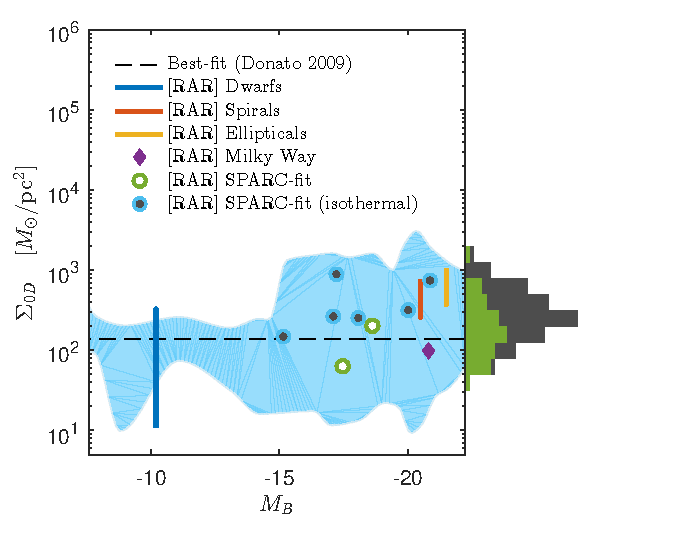
\includegraphics[width=\hsize]{\ROOTPATH/fig.pdf}
	\caption{Radial acceleration curve of NGC0055 with SPARC data (circles), McGaugh's empirical fit (dashed line, see \cref{egn:mcgaugh-fit}) and best fits of the considered DM models. The dotted line shows where dark matter and baryonic accelerations are equal. RAR and DC14 produce very similar results while NFW is disfavored here (compare \cref{fig:RC:NGC0055}).}%
\label{fig:AC:NGC0055}
\end{figure}